% \chapter{Uncertainty and Error Propagation}
\chapter{不确定性和误差传播}
\label{chap:uncertainty}

% Robots are systems that combine sensing, actuation, computation, and communication. Except for computation, all of its sub-systems are subject to a high degree of uncertainty. This can be observed in daily life: phone calls often are of poor quality, making it hard to understand the other party, characters are difficult to read from far away,  the front wheels of your car slip when accelerating on a rainy road from a red light, or your wireless device has a hard time getting a connection. In robotics, measurements taken by on-board sensors are sensitive to changing environmental conditions and subject to electrical and mechanical limitations. Similarly, actuators are not accurate as joints and gears have backlash and wheels do slip. Finally, communication, in particular, wireless either via radio or infrared, is notoriously unreliable.

% The goals of this chapter are to understand

机器人是结合感测,致动,计算和通信的系统。除计算外,其所有子系统均处于高度不确定状态。这可以在日常生活中观察到:电话通常质量差,使得很难理解对方,人物很难从远处读取,汽车的前轮在从红色的雨道加速时滑落光或无线设备很难获得连接。在机器人技术中,车载传感器采取的测量对变化的环境条件敏感,并受到电气和机械限制。类似地,执行器不准确,因为关节和齿轮具有齿隙并且轮子滑动。最后,通信,特别是通过无线电或红外线的无线通信是众所周知的不可靠的。

本章的目标是要了解

\begin{itemize}
% \item how to treat uncertainty mathematically using probability theory,
% \item how measurements with different uncertainty can be combined,
% \item how error propagates when taking multiple measurements in a row.

\item 如何使用概率论数学地处理不确定性,
\item 如何组合不同不确定度的测量,
\item 在连续进行多个测量时如何传播错误。
\end{itemize}

% This chapter requires an understanding of random variables, probability density functions, and in particular the Normal distribution. These concepts are explained in a robotic sensing context in Appendix \ref{sec:pdfs}. 

本章需要了解随机变量,概率密度函数,特别是正态分布。这些概念在附录\ref{sec:pdfs}中的机器人感应环境中解释。

% \section{Uncertainty in Robotics as Random Variable}
% As quantities such as ``distance to a wall", ``position on the plane'' or ``I can see a blue cross (yes/no)'' are uncertain, we can consider them random variables. A \emph{random variable}\index{Random Variable} can be thought of us the outcome of a ``random'' experiment, such as the face shown when throwing a dice. 

% Experiments in robotics rarely involve explicit randomness. Instead, sensors are intrinsically noisy due to the physical phenomena associated with them. As sensor readings therefore can be considered random variables, also quantities derived from one or more sensors, such as the examples above, are random variables. This chapter focusses on how to characterize the uncertainty of such aggregated quantities from the uncertainty that characterizes the individual sensors. 

\section{机器人中的不确定性作为随机变量}
由于“距离墙”,“飞机上的位置”或“我可以看到蓝色十字架(是/否)”的数量是不确定的,我们可以考虑它们随机变量。\emph{随机变量}\index{Random Variable}可以被认为是“随机”实验的结果,例如投掷骰子时所显示的面。

机器人实验很少涉及明显的随机性。相反,由于与它们相关的物理现象,传感器本质上是嘈杂的。因此,由于传感器读数因此可以被认为是随机变量,所以从一个或多个传感器得到的量也是随机变量。本章重点介绍如何从表征各个传感器的不确定性来表征这些聚合量的不确定性。

% \section{Error Propagation}
\section{误差传播}
\label{sec:errorprop}

% It turns out that the Gaussian Distribution is very appropriate to model prominent random processes in robotics: the robot's position and distance measurements. A differential wheel robot that drives along a straight line, and is subject to slip, will actually increase its uncertainty the farther it drives. Initially at a known location, the expected value (or mean) of its position will be increasingly uncertain, corresponding to an increasing variance. This variance is obviously somehow related to the variance of the underlying mechanism, namely the slipping wheel and (comparably small) encoder noise. Interestingly, we will see its variance grow much faster orthogonal to the robot's direction, as small errors in orientation have a much larger effect than small errors in longitudnal direction. This is illustrated in Figure \ref{fig:errorprop_odometry}. 

事实证明,高斯分布非常适合于模拟机器人中突出的随机过程:机器人的位置和距离测量。沿着直线驱动并受到滑动的差速器轮机器人实际上将增加其驱动的更远的不确定性。最初在一个已知的位置,其位置的预期值(或平均值)将越来越不确定,对应于增加的方差。这种差异显然与底层机制的方差有关,即滑轮和(相对小的)编码器噪声。有趣的是,我们将看到它的方差正比于机器人的方向变化更快,因为方向上的小误差比纵向方向上的小误差具有更大的影响。这在图\ref{fig:errorprop_odometry}中说明。

\begin{figure}
	\centering
		\includegraphics[width=\textwidth]{figs/errorprop_odometry}
	% \caption{Two-dimensional Normal distribution depicting growing uncertainty as the robot moves. Albeit starting with equal uncertainty in $x$ and $y$, the large effect of small errors in orientation let the error grow faster in y-direction of the robot.}
	\caption{二维正态分布描述了机器人移动时的不确定性。尽管从$x$和$y$中的相等的不确定性开始,定向中的小错误的巨大影响使得错误在机器人的y方向上增长更快。}
	\label{fig:errorprop_odometry}
\end{figure}

% Similarly, when estimating distance and angle to a line feature from point cloud data, the uncertainty of the random variables describing distance and angle to the line are somewhat related to the uncertainty of \emph{each} point measured on the line. These relationships are formally captured by the \emph{error propagation law}\index{Error Propagation Law}.

% The key intuition behind the error propagation law is that the variance of each component that contributes to a random variable should be weighted as a function of how strongly this component influences this random variable. Measurements that have little effect on the aggregated random variable should also have little effect on its variance and vice versa. ``How strongly'' something affects something else can be expressed by the ratio of how little changes of something relate to little changes in something else. This is nothing else than the partial derivative of something with respect to something else. For example, let $y=f(x)$ be a function that maps a random variable $x$, e.g., a sensor reading, to a random variable $y$, e.g., a feature. Let the standard deviation of $x$ be given by $\sigma_x$. We can then calculate the variance $\sigma_y^2$ by 

类似地,当从点云数据估计与线特征的距离和角度时,描述与线的距离和角度的随机变量的不确定性与在线测量的\emph{each}点的不确定性有些相关。这些关系由\emph{errorpropagationlaw}\index{ErrorPropagationLaw}正式捕获。

错误传播规律背后的关键直觉是,有助于随机变量的每个组件的方差应该被加权作为这个组件影响这个随机变量的强度的函数。对聚合随机变量几乎没有影响的测量对其方差也应该没有什么影响,反之亦然。某些东西影响其他东西的“多么强烈”可以通过某些事物的变化与其他事物的微小变化的比例来表达。这不是别的东西的偏导数。例如,让$y=f(x)$是将随机变量$x$(例如,传感器读数)映射到随机变量$y$(例如特征)的函数。让$x$的标准偏差由$\sigma_x$给出。然后,我们可以计算方差$\sigma_y^2$


\begin{equation}
\sigma_y^2=\left(\frac{\partial f}{\partial x}\right)^2 \sigma_x^2
\end{equation}

% In case $\mathbf{y}=f(\mathbf{x})$ is a multivariable function that maps $n$ inputs to $m$ outputs, variances become covariance \emph{matrices}. A covariance matrix holds the variance of each variable along its diagonal and is zero otherwise, if the random variables are not correlated. We can then write

如果$\mathbf{y}=f(\mathbf{x})$是将$n$输入映射到$m$输出的多变量函数,则方差变为协方差\emph{matrices}。协方差矩阵保持每个变量沿其对角线的方差,否则,如果随机变量不相关。然后我们可以写

\begin{equation}
\Sigma^Y= J \Sigma^X J^T
\end{equation}

% where $\Sigma^X$ and $\Sigma^Y$ are the covariance matrices holding the variances of the input and output variables, respectively, and $J$ is a $m$x$n$ \emph{Jacobian} matrix, which holds the partial derivatives $\frac{\partial f_i}{\partial x_j}$. As $J$ has $n$ columns, each row contains partial derivatives with respect to $x_1$ to $x_n$.

其中$\Sigma^X$和$\Sigma^Y$分别是保存输入和输出变量的方差的协方差矩阵,$J$是一个$m$x$n$\emph{Jacobian}矩阵,它保存偏导数$\frac{\partial f_i}{\partial x_j}$。由于$J$有$n$列,每行包含关于$x_1$至$x_n$的偏导数。

% \subsection{Example: Line Fitting}
\subsection{示例:线拟合}
\label{sec:linefitting}

% Lets consider an example of estimating angle $ \alpha$ and distance $ r$ of a line from a set of points given by $ (\rho_i,\theta_i)$ using Equations \ref{eq:linealpha}--\ref{eq:liner}. We can now express the relationship of changes of a variable such as $ \rho_i$ to changes in $ \alpha$ by

让我们考虑一个例子,从$(\rho_i,\theta_i)$给出的一组点估计一个线的角度$\alpha$和距离$r$,使用方程\ref{eq:linealpha}-\ref{eq:liner}。现在我们可以将变量$\rho_i$的变化与$\alpha$中的变化表达出来

\begin{equation}
\frac{\partial \alpha}{\partial \rho_i}
\end{equation}

% Similarly, we can calculate $ \frac{\partial \alpha}{\partial \theta_i}$, $ \frac{\partial r}{\partial \rho_i}$ and $ \frac{\partial r}{\partial \theta_i}$. We can actually do this, because we have derived analytical expressions for $ \alpha$ and $ r$ as a function of $ \theta_i$ and $ \rho_i$ in Chapter \ref{chap:feature_extraction}.

% We are now interested in deriving equations for calculating the variance of $ \alpha$ and $ r$ as a function of the variances of the distance measurements. Lets assume each distance measurement $ \rho_i$ has variance $ \sigma^2_{\rho_i}$ and each angular measurement $ \theta_i$ has variance $ \sigma^2_{\theta_i}$. We now want to calculate $ \sigma^2_{\alpha}$ as the weighted sum of  $ \sigma^2_{\rho_i}$ and $ \sigma^2_{\theta_i}$, each weighted by its influence on $ \alpha$.

% More generally, if we have $ I$ input variables $ X_i$ and $ J$ output variables $Y_j$, the covariance matrix of the output variables $ \sigma_Y$ can be expressed as $\sigma_Y^2=\frac{\partial f}{\partial X}^2 \sigma_X^2$ where $\sigma_X$ is the covariance matrix of input variables and $J$ is a Jacobian matrix of a function $ f$ that calculates $Y$ from $X$ and has the form

类似地,我们可以计算$\frac{\partial\alpha}{\partial\theta_i}$,$\frac{\partial r}{\partial\rho_i}$和$\frac{\partial r}{\partial\theta_i}$。我们实际上可以做到这一点,因为我们已经将$\alpha$和$r$的解析表达式作为$\theta_i$和$\rho_i$在第\ref{chap:feature_extraction}中的函数。

我们现在有兴趣得出方程来计算$\alpha$和$r$的方差,作为距离测量的方差的函数。让我们假定每个距离测量$\rho_i$有方差$\sigma^2_{\rho_i}$和每个角度测量$\theta_i$有方差$\sigma^2_{\theta_i}$。我们现在要计算$\sigma^2_{\alpha}$作为$\sigma^2_{\rho_i}$和$\sigma^2_{\theta_i}$的加权和,$\alpha$。

更一般地说,如果我们有$I$输入变量$X_i$和$J$输出变量$Y_j$,输出变量$\sigma_Y$的协方差矩阵可以表示为$\sigma_Y^2=\frac{\partial f}{\partial X}^2\sigma_X^2$其中$\sigma_X$是输入变量的协方差矩阵,$J$是从$X$计算$Y$的函数$f$的雅可比矩阵,有形式

\begin{equation}
J=\left[
\begin{array}{ccc}
  \frac{\partial f_1}{\partial X_1} & \ldots & \frac{\partial f_1}{\partial X_I}\\
  \vdots & \ldots & \vdots\\
  \frac{\partial f_J}{\partial X_1} & \ldots & \frac{\partial f_J}{\partial X_I}
 \end{array}
 \right]
\end{equation}

% In the line fitting example $ F_X$ would contain the partial derivatives of $ \alpha$ with respect to all $ \rho_i$ (i-entries) followed by the partial derivates of $ \alpha$ with respect to all $ \theta_i$ in the first row. In the second row, $ F_X$ would hold the partial derivates of $ r$ with respect to $ \rho_i$ followed by the partial derivates of $ r$ with respect to $ \theta_i$. As there are two output variables, $ \alpha$ and $ r$, and 2*I input variables (each measurement consists of an angle and distance), $ F_X$ is a 2 x (2I) matrix.

% The result is therefore a 2x2 covariance matrix that holds the variances of $ \alpha$ and $ r$ on its diagonal.

在线拟合示例中,$F_X$将包含相对于所有$\rho_i$(i条目)的$\alpha$的偏导数,后跟$\alpha$的偏导数相对于所有$\theta_i$第一行。在第二行,$F_X$将保存相对于$\rho_i$的$r$的部分派生,后跟相对于$\theta_i$的$r$的部分派生。由于有两个输出变量$\alpha$和$r$和2*I输入变量(每个测量由一个角度和距离组成),$F_X$是一个2x(2I)矩阵。

因此,结果是2x2协方差矩阵,其在对角线上保存$\alpha$和$r$的差异。

% \subsection{Example: Odometry}
\subsection{示例:里程计}
\screencast{https://www.youtube.com/watch?v=ubg_AAM7Zd8}{errorpropagation}

% Whereas the line fitting example demonstrated a many-to-one mapping, odometry requires to calculate the variance that results from multiple sequential measurements.  Error propagation allows us here to not only express the robot's position, but also the variance of this estimate. Our ``laundry list'' for this task looks as follows:

而线拟合示例演示了多对一映射,测距需要计算由多个连续测量结果产生的方差。错误传播允许我们在这里不仅表达机器人的位置,而且还表示这个估计的方差。我们对这个任务的“洗衣单”看起来如下:

\begin{enumerate}
% \item What are the input variables and what are the output variables?
% \item What are the functions that calculate output from input?
% \item What is the variance of the input variables?

\item 什么是输入变量,什么是输出变量?
\item 从输入计算输出的函数是什么?
\item 输入变量的方差是多少?
\end{enumerate}

% As usual, we describe the robot's position by a tuple $ (x,y,\theta)$. These are the three output variables. We can measure the distance each wheel travels $ \Delta s_r$ and $ \Delta s_l$ based on the encoder ticks and the known wheel radius. These are the two input variables. We can now calculate the change in the robot's position by calculating

像往常一样,我们通过元组$(x,y,\theta)$来描述机器人的位置。这些是三个输出变量。我们可以根据编码器刻度和已知的车轮半径来测量每个车轮行驶的距离$\Delta s_r$和$\Delta s_l$。这些是两个输入变量。我们现在可以通过计算来计算机器人位置的变化

\begin{eqnarray}
\Delta x  &=& \Delta s cos(\theta+\Delta \theta /2)\\
\Delta y  &=& \Delta s sin(\theta+\Delta \theta/2)\\
\Delta \theta &=& \frac{\Delta s_r-\Delta s_l}{2}
\end{eqnarray}
% with
和

\begin{equation}
\Delta s=\frac{\Delta s_r + \Delta s_l}{2}
\end{equation}

% The new robot's position is then given by

然后给出新的机器人的位置
\begin{equation}
f(x,y,\theta,\Delta s_r, \Delta s_l)=[x,y,\theta]^T + [\Delta x \qquad \Delta y \qquad \Delta \theta]^T
\end{equation}


% We thus have now a function that relates our measurements to our output variables. What makes things complicated here is that the output variables are a function of their previous values. Therefore, their variance does not only depend on the variance of the input variables, but also on the previous variance of the output variables. We therefore need to write

因此,我们现在有一个功能将我们的测量与我们的输出变量相关联。这使得事情变得复杂的是输出变量是其先前值的函数。因此,它们的差异不仅取决于输入变量的方差,还取决于输出变量的先前方差。所以我们需要写

\begin{equation}\label{eq:errorpropodom}
\Sigma_{p'}=\nabla_p f \Sigma_p \nabla_p f^T + \nabla_{\Delta_{r,l}}f \Sigma_{\Delta}\nabla_{\Delta_{r,l}}f^T
\end{equation}

% The first term is the error propagation from a position $ p=[x,y,\theta]$ to a new position $ p'$. For this we need to calculate the partial derivatives of $ f$ with respect to x, y and $ \theta$. This is a 3x3 matrix

第一个术语是从位置$p=[x,y,θ]$到新位置$p'$的错误传播。为此,我们需要计算相对于x,y和$\theta$的$f$的偏导数。这是一个3x3矩阵

\begin{equation}
\nabla_p f=\left[\frac{\partial f}{\partial x} \quad \frac{\partial f}{\partial y} \quad \frac{\partial f}{\partial \theta}\right]=\left[\begin{array}{ccc}1 & 0 & -\Delta s sin(\theta +\Delta \theta /2)\\0 & 1 & \Delta s cos(\theta + \Delta \theta/2)\\0 & 0 &1\end{array}\right]
\end{equation}

% The second term is the error propagation of the actual wheel slip. This requires calculating the partial derivatives of $ f$ with respect to $ \Delta s_r$ and $ \Delta s_l$, which is a 3x2 matrix. The first column contains the partial derivatives of $ x,y,\theta$ with respect to $ \Delta s_r$. The second column contains the partial derivatives of $ x,y,\theta$ with respect to $ \Delta s_l$:

第二项是实际车轮滑差的误差传播。这需要计算相对于$\Delta s_r$和$\Delta s_l$(它是3x2矩阵)的$f$的偏导数。第一列包含$x,y,\theta$相对于$\Delta s_r$的偏导数。第二列包含$x,y,\theta$相对于$\Delta s_l$的偏导数:

\begin{equation}
\nabla_{\Delta_{r,l}} f=\left[
\begin{array}{cc}
\frac{1}{2}\cos(\theta+\Delta \theta/2) & \frac{1}{2}\cos(\theta+\Delta \theta/2)\\
\frac{1}{2}\sin(\theta+\Delta \theta/2) & \frac{1}{2}\cos(\theta+\Delta \theta/2)\\
\frac{1}{2} & -\frac{1}{2}
\end{array}
\right]
\end{equation}

% Finally, we need to define the covariance matrix for the measurement noise. As the error is proportional to the distance travelled, we can define $ \Sigma_{\Delta}$ by

最后,我们需要定义测量噪声的协方差矩阵。由于误差与行进距离成比例,我们可以定义$\Sigma_{\Delta}$

\begin{equation}
\Sigma_{\Delta}=\left[\begin{array}{cc}k_r|\Delta s_r| & 0\\0 & k_l|\Delta s_l|\end{array}\right]
\end{equation}


% Here $ k_r$ and $ k_l$ are constants that need to be found experimentally and $ |\cdot |$ indicating the absolute value of the distance traveled. We also assume that the error of the two wheels is independent, which is expressed by the zeros in the matrix.

% We now have all ingredients for equation \ref{eq:errorpropodom}, allowing us to calculate the covariance matrix of the robot's pose much like shown in Figure \ref{fig:errorprop_odometry}.


这里$k_r$和$k_l$是需要在实验中找到的常量,$|\cdot|$表示行进距离的绝对值。我们还假设两个轮子的误差是独立的,这是由矩阵中的零表示的。

我们现在拥有等式\ref{eq:errorpropodom}的所有成分,使我们能够计算机器人姿态的协方差矩阵,如图所示\ref{fig:errorprop_odometry}。


% \section{Take-home lessons}
\section{课后补充}

\begin{itemize}
% \item Uncertainty can be expressed by means of a probability density function.
% \item More often than not, the Gaussian distribution is chosen as it allows treating error with powerful analytical tools.
% \item In order to calculate the uncertainty of a variable that is derived from a series of measurements, we need to calculate a weighted sum in which each measurement's variance is weighted by its impact on the output variable. This impact is expressed by the partial derivative of the function relating input to output.

\item 不确定度可以通过概率密度函数来表示。
\item 通常选择高斯分布,因为它可以通过强大的分析工具处理错误。
\item 为了计算从一系列测量中导出的变量的不确定性,我们需要计算加权和,其中每个测量的方差对其对输出变量的影响加权。 这种影响由与输出相关的函数的偏导数表示。
\end{itemize}

\section*{Exercises}\small
\begin{enumerate}
% \item Given two observations $\hat{q}_1$ and $\hat{q}_2$ with variances $\sigma_1$ and $\sigma_2$ of a normal distributed process with actual value $\hat{q}$, an optimal estimate can be calculated by minimizing the expression

\item 给出两个观察值$\hat{q}_1$和$\hat{q}_2$,具有实际值$\hat{q}$的正态分布式进程的差异$\sigma_1$和$\sigma_2$,可以通过最小化表达式来计算最优估计

\begin{equation}
\nonumber
S=\frac{1}{\sigma_1^2}(\hat{q}-\hat{q}_1)^2+\frac{1}{\sigma_2^2}(\hat{q}-\hat{q}_2)^2
\end{equation}

% Calculate $\hat{q}$ so that $S$ is minimized.
计算$\hat{q}$,使$S$最小化。

% \item An ultrasound sensor measures distance $x=c\Delta t/2$. Here, $c$ is the speed of sound and $\Delta t$ is the difference in time between emitting and receiving a signal.

\item 超声波传感器测量距离$ x = c \ Delta t / 2 $。 这里,$ c $是声音的速度,$ tt $是发射和接收信号之间的时间差。

\begin{enumerate}
% \item Let the variance of your time measurement $\Delta t$ be $\sigma_t^2$. What can you say about the variance of $x$, when $c$ is assumed to be constant? Hint: how does a change in $\Delta t$ affect $x$?
% \item Now assume that also $c$ is changing depending on location, weather, etc. and can be estimated with variance $\sigma_c^2$. What is the variance of $x$ now?

\item 让你的时间测量的方差$\Delta t$为$\sigma_t^2$。当$c$被假定为常数时,您可以对$x$的方差说些什么?提示:$\Delta t$中的更改如何影响$x$?
\item 现在假设$c$根据位置,天气等而改变,并且可以用方差$\sigma_c^2$估计。现在$x$的差异是多少?
\end{enumerate}
% \item Consider a unicycle that turns with angular velocity $\dot{\phi}$ and has radius $r$. Its speed is thus a function of $\dot{\phi}$ and $r$ and is given by

\item 考虑以角速度$\dot{\phi}$转动并且具有半径$r$的独轮车。它的速度因此是$\dot{\phi}$和$r$的函数,由给出

\begin{equation}
\nonumber
v=f(\dot{\phi},r)=r\dot{\phi}
\end{equation} 
% Assume that your measurement of $\dot{\phi}$ is noisy and has a standard deviation $\sigma_{\phi}$.  Use the error propagation law to calculate the resulting variance of your speed estimate $\sigma_v^2$. 

假设您的$\dot{\phi}$的测量值是嘈杂的,并具有标准偏差$\sigma_{\phi}$。使用误差传播规律计算您的速度估计值$\sigma_v^2$的结果方差。

\end{enumerate}
\normalsize
